\subsection{Grafo}

\begin{frame}
    \frametitle{Grafo - Repaso}

    Las bases de datos en grafo utilizan estructuras de grafo para almacenar, consultar y relacionar datos. 

     
    
    \begin{columns}
        \begin{column}{0.48\textwidth}
            Los datos se representan mediante nodos (entidades) y arcos (relaciones entre entidades).
        \end{column}
        \begin{column}{0.48\textwidth}
            \centering
            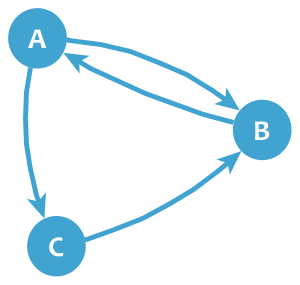
\includegraphics[width=0.4\textwidth]{images/Grafo.png}
        \end{column}
    \end{columns}

     

    \vspace{0.3cm}
    
    Pueden asignarse propiedades a nodos y arcos para capturar más detalles.

     
    
    Son ideales para almacenar datos interconectados.  

     
    
    Aplicaciones comunes incluyen: \textbf{Redes sociales}, \textbf{Sistemas de recomendación}, \textbf{Redes de trasportes}, etc.

    
\end{frame}

\begin{frame}
    \frametitle{Grafo - Ejemplos}

    Algunos ejemplos de bases de datos en grafos son:

    \begin{itemize}
        \item \textbf{Neo4j}\\
         
        \item \textbf{GraphBase}\\ 

        \item \textbf{Infinite Graph}\\
        
        \item \textbf{FlockDB}\\
    \end{itemize}
    
     

    Nos vamos a centrar en Neo4j.
    
\end{frame}

\subsubsection{Neo4j}

\begin{frame}
    \frametitle{Grafo - Neo4j}

    \centering
    
\includegraphics[width=0.5\textwidth]{images/neo4j-logo.png}

    \begin{itemize}
        \item Plataforma líder en bases de datos de grafos.  
        \item Diseño nativo de grafo para un rendimiento óptimo y escalabilidad excepcional.  
        \item Utiliza Cypher como su lenguaje de consulta principal.  
        \item Ofrece una interfaz integrada de visualización de grafos.  
        \item Altamente escalable y diseñado para manejar grandes volúmenes de datos.  
        \item Garantiza propiedades ACID.  
        \item Edición empresarial.
    \end{itemize}
    
\end{frame}

\begin{frame}{Cypher: Lenguaje de Consulta de Neo4j}
    \begin{itemize}
        \item Sintaxis intuitiva y expresiva.  
        \item Orientado a patrones.  
        \item Declarativo.  
        \item Soporte completo para operaciones CRUD.  
        \item Amplio soporte para funciones y operadores para operaciones avanzadas.
    \end{itemize}
\end{frame}

\begin{frame}
    \frametitle{Operaciones Básicas de Neo4j}

    Estas son algunas de las cláusulas básicas más comunes en Cypher y su sintaxis asociada:

     

    \begin{itemize}
        \item \textbf{Crear nodos y relaciones}

        \texttt{CREATE (a:Person \{name: 'John', age: 30\})} \newline
         
        \texttt{CREATE (b:Person:Employee 
                            \{name: 'Alice', role: 'Manager'\})}\newline
         
        \texttt{CREATE (a)-[:FRIENDS\_WITH]->(b)}

         
            
        \item \textbf{Especificar patrones}
        
        \texttt{MATCH (p:Person \{name: 'John'\}) RETURN p}\newline
         
        \texttt{MATCH (p:Person \{name: 'John'\})-[r]->() RETURN p, r}

         
    
    
        \item \textbf{Filtrar resultados}

        \texttt{WHERE n.name = 'John' AND friend.age > 25}

 
    \end{itemize}
    
\end{frame}

\begin{frame}
    \frametitle{Operaciones Básicas de Neo4j}


    \begin{itemize}

     
        \item \textbf{Devolver datos}

        \texttt{RETURN n, friend}

         
         
        \item \textbf{Actualizar propiedades}

        \texttt{SET n.age = 30}

         
        
        \item \textbf{Eliminar nodos y relaciones.}

        \texttt{DELETE n, friend}

         
            
        \item \textbf{Ordenar resultados}

        \texttt{ORDER BY n.name DESC}

         
        
        \item \textbf{Limitar número de resultados}

        \texttt{LIMIT 10}

         

        \item \textbf{Crear índices}

        \texttt{CREATE INDEX ON :Person(name)}
    
        
    \end{itemize}
    
\end{frame}

\begin{frame}[fragile]
  \frametitle{Ejemplo de Consulta en Neo4j}
      Para una demostración de como estas operaciones podrían ser utilizadas, supongamos que queremos encontrar los amigos en común entre dos usuarios en una red social y alguna información adicional sobre esos amigos en común:  
    \begin{verbatim}
MATCH (userA:User {username: 'UsuarioA'})
    -[:FRIENDS_WITH]-(commonFriend)-[:FRIENDS_WITH]-
    (userB:User {username: 'UsuarioB'})
RETURN commonFriend.username AS commonFriendUsername,
       commonFriend.age AS commonFriendAge
    \end{verbatim}

        
\end{frame}

\begin{frame}{Empresas que Utilizan Neo4j}
    \begin{itemize}
        \item Walmart
        \item Volvo
        \item eBay
        \item Cisco
    \end{itemize}
\end{frame}